\documentclass[colorlinks=true,pdfstartview=FitV,linkcolor=blue,
            citecolor=magenta,urlcolor=red]{ligodoc}

\usepackage{graphicx}
\usepackage{hyperref}
\usepackage{amssymb}
\usepackage{amsmath}
\usepackage{longtable}
\usepackage{float}
\usepackage{rotating}
\usepackage[usenames,dvipsnames]{color}
\usepackage{fancyhdr}
\usepackage{subcaption}

\graphicspath{{figures/}}

%%%%%%%%%%%%%%%%%%%%%%%%%%%%%%
\title{Conditioning ring heater actuator input to optimize thermo-optic response}
\author{Daniel Vander-Hyde, Stefan Ballmer}
%\date{${}$Date: 2007/09/30}
\ligodccnumber{T}{19}{00496}{v0}{D} \ligodistribution{LIGO Scientific Collaboration}
%\ligodraft

%%%%%%%%%%%%%%%%%%%%%%%%%%%%%%%%%%%%%%%%%%%%%%%%%%%%%%%%%%%%%%%%%%%%%
\begin{document}

%%%%%%%%%%%%%%%%%%%%%%%%%%%%%%%%%%%%%%%%%%%%%%%%%%%%%%%%%%%%%%%%
\section{Overview}
\label{sec:I}
As the Advanced LIGO detectors reach $\approx$ 200kW of circulating power in the Fabry Perot arm cavities, ring heater actuation becomes cruicial for O3 comissioning and to achieve a required thermo-optic lens by adjusting the ring heater (RH) acutators it may take on the order of 10-12 hours (Fig \ref{fig:meas}) to reach a steady thermal lens. This response after RH adjustement results in a large amount of time the interferometer will be improperly mode matched, making the adjustment of thermal compensation a laborious process. The thermo-optic step response of the LIGO test mass / ring heater system can be shortened to 2-4 hours with real time digital filtering of the ring heater actuator power input. The following sections describe the concept and design of contructing the real-time digital filter.


\begin{figure}[H]
 \includegraphics[width=\textwidth]{python/Meas_response}
 \caption{ITMY thermo-optic response to a 3.13 Watt power reduction to ring heaters. It's after $\approx$ 12 hours after the change was made do you start to see a small enough $\frac{\mathrm{d} \alpha_\mathrm{sp}}{\mathrm{dt}}$ when you can assume a steady thermal lens.}
 \label{fig:meas}
\end{figure}
%%%%%%%%%%%%%%%%%%%%%%%%%%%%%%%%%%%%%%%%%%%%%%%%%%%%%%%%%%%%%%%%%%%%%
%\newpage
\section{Concept}
\label{sec:III}

Before this method was implemented at the LIGO Hanford and Livingston sites, ring heater settings were adjusted by stepping the ring heater to a desired power though the thermo-optic step response function (H(s)) of the RH (Fig [\ref{fig:meas}]) shows the ITMY RH response for an approximate 10 hour period after your RH input power is changed,  $\frac{\mathrm{d}\alpha_{\mathrm{sp}}}{\mathrm{dt}}$ is nonzero. This long response time can be attributed to undermanaged heat being injected through the optic by stepping the power to the RH actuators.

\begin{figure}[H]
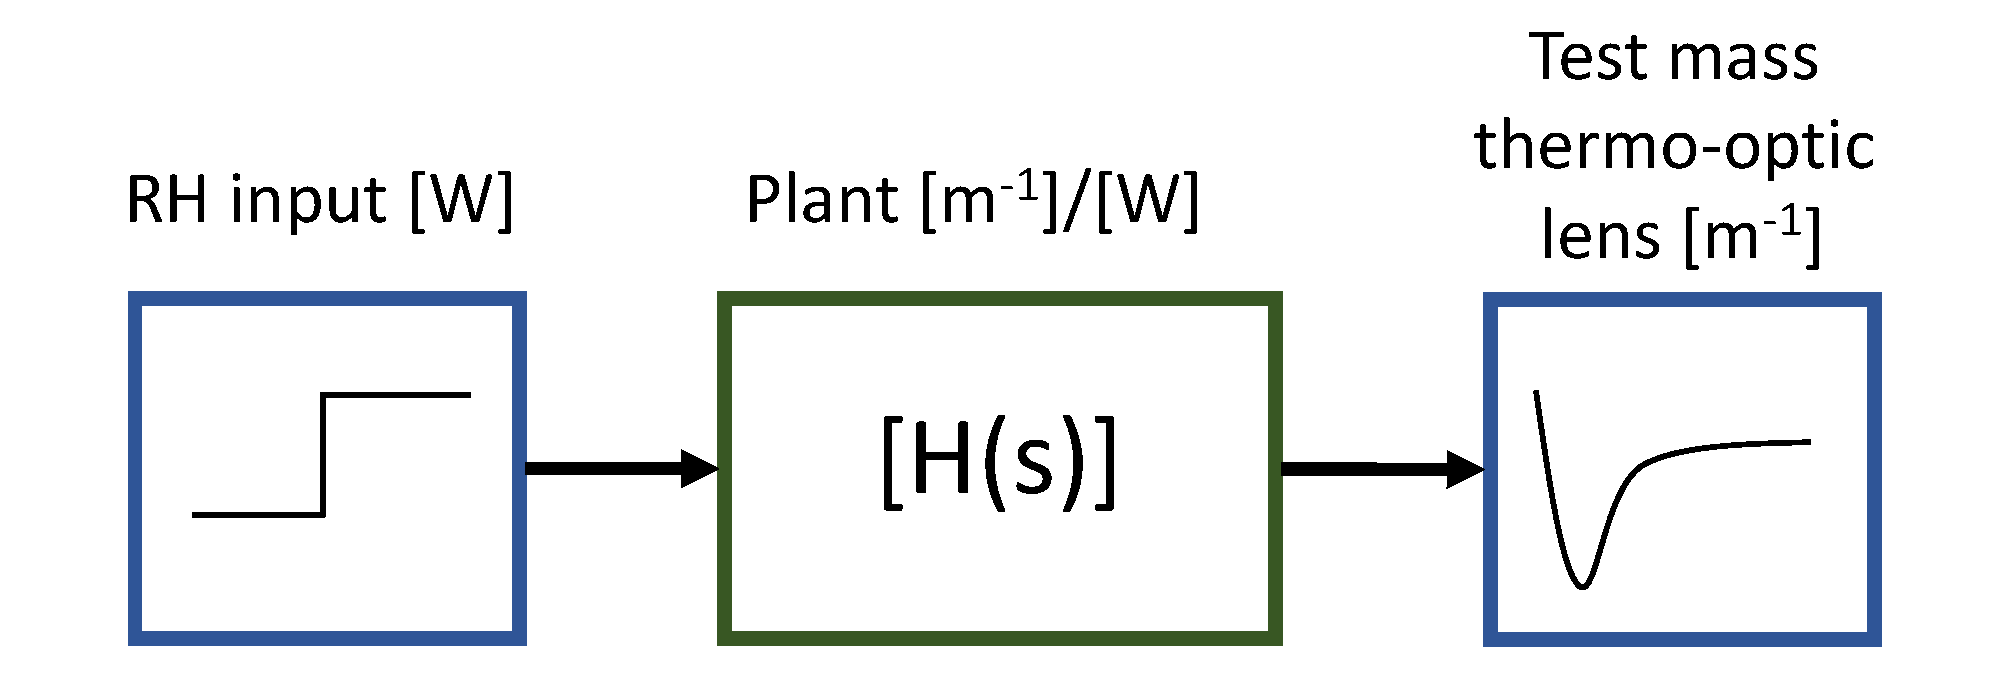
\includegraphics[page=1,width=\textwidth]{RH_input_filter_figures.pdf}
\caption{A pictograph showing how the plant transforms the signal. The example of this can be seen in Fig [\ref{fig:meas}]}
\label{fig:justplant}
\end{figure}

For the most optimal management of injected RH power to the optic over time, constructing a real time digital filter custom made from the plant model (H(s)) will be critical to increasing the convergence speed of the RH/optic response. The first component to constructing this input RH filter ($[\mathrm{H}(\mathrm{s})]^{-1*}$) is inverting the ring heater thermo-optic step response. As will be seen in the next section, this suggests an unstable filter which motivates us to modify the inverse plant filter hence the asterisk in $[\mathrm{H}(\mathrm{s})]^{-1*})$.

\begin{figure}[H]
\includegraphics[page=2,width=\textwidth]{RH_input_filter_figures.pdf}
\caption{A pictograph showing the system with real time digital filtering for an improved thermo-optic response. The RH input filter is created by inverting the plant filter combine with a low pass and added poles to the zpk model to ensure stability. }
\label{fig:plantwfilt}
\end{figure}



\section{Initial Filter Design}
\subsection{Plant filter (H(s))}

The plant filter was acquired by transforming the computed impulse response from [\ref{fig:meas}] into the Laplace domain and hand fitting a zpk filter over it.

\begin{figure}[H]
\includegraphics[width=\textwidth]{python/RH_plant_filter_fit}
\caption{A comparison between the plant filter acquired from the measured ITMY RH step response data and the hand fitted H(s).}
\label{fig:plantfilt}
\end{figure}

The fitted zpk filter for ITMY is a one zero / three pole filter:


$$ H(s) = 9.2545*10^{-12} \frac{(s+3.142*10^{-5})}{(s+ 8.168*10^{-5}) (s+0.0003142) (s+0.0005969)} $$


\subsection{Inverse Plant filter (H$^{-1}$(s))}
\begin{figure}[H]
\includegraphics[width=\textwidth]{python/RH_inv_filt}
\caption{Inverted plant filter H$^{-1}$(s)}
\label{fig:inv_plant_filt}
\end{figure}

$$ H^{-1}(s) = \frac{1}{9.2545*10^{-12}} \frac{(s+ 8.168*10^{-5}) (s+0.0003142) (s+0.0005969)}{(s+3.142*10^{-5})} $$

By just inverting the filter we have constructed a filter with a logarithmic rise in gain after .1 mHz. Implementing this filter without further modification would lead to high frequency artifacts in your ring heater power time series, suggesting a non-optimal response. Further modification is needed.

\newpage

\subsection{Ring Heater input filter (Real time digital filter) ([H$^{-1}$(s)]$^{*}$)}
An important modification was made after inverting the filter: 2 poles were added at -.0007 Hz to the same level of gain at DC ($<10^{-6}$Hz). This limit to the filter is necessary to reassure stability at .1 mHz.

\begin{figure}[H]
\includegraphics[width=\textwidth]{python/RH_input_filt}
\caption{The final form of the input RH filter for the ITMY RH.}
\label{fig:inv_plant_filt_mod}
\end{figure}

$$ [H^{-1}(s)]^{*} = \frac{(s+8.168*10^{-5}) (s+0.0003142) (s+0.0005969)}{(s+3.142*10^{-5}) (s+0.0006994)^2} $$


\newpage
\subsection{Testing}
\subsubsection{Expected Performance}

\begin{figure}[H]
\includegraphics[width=\textwidth]{python/IRHF_step_vs_filt_step}
\caption{Comparison of the natural RH response and the response to the conditioned input. The above plot is simulated in Matlab by passing the RH input time series (top plot) through the $[H^{-1}(s)]*G(s)$ and $H(s)$ to acquire with the result lensing behavior on the bottom plot.}
\label{fig:comparison}
\end{figure}



\subsubsection{RH measurement at LHO}
Figure (?) demonstrates the performance of the filter for a ? W change of the RH at LHO:



\section{Limitations}
Though the RH does reduce the mirror ROC convergence time by nearly a factor of 6, there needs to be discussion about the limitations of the filter. When inverting this filter you might imagine that we are demanding the most step-like thermo-optic response from our initial plant H(s). Therefore this could imply (look into this) that any more energy injected into the system would imply overshoot while any less would imply an undershoot, but it turns out that if you incorporate the much larger RH range. In a way the inversion suggests the most optimal time series.  This being said, we also must demand that the system remain stable in this chain of filters which requires that we limit the gain so that $[H^{-1}(s)]^{*} \leq 1$ for $Re(s)/(2*\pi)>.1 \mathrm{mHz}$.


\section{Dynamic Thermal Compensation and Limitations}
At LLO mitigating the ROC change due to the central self heating transient is achieved through dynamic thermal compensation by adjustment of the RH actuators (at LHO it is achieved by reducing (central) CO2 heating) [refs] (alogs and TVo's thesis). The problem using the above real time digital filter can be with the above response, which is at a time scale is still significantly longer ($\approx 2.5\;\mathrm{hrs}$) than the (central) self heating of the test masses from the interferometer beam ($\approx 1\; \mathrm{hr}$).

Making the assumption that the plant filter still applies for large RH power and that the largest actuation power that the RHs can supply can go up to 40W, we extend the above method to attempt to compensate the central lensing caused by self heating of the interferometer beam. This quick mirror geometry adjustement not only proves to be useful for maintaining coupled cavity mode matching also helps mitigate parametric instabilities PI [ref Terra's paper].

Given this model, we demonstrate that this thermal compensation technique may only be used for up to \textbf{$\approx$ 400 kW of circulating arm power}.

\subsection{Limitations}
Though in principle this fast actuation behavior can be done, it is still hard to say whether it will be a strain to the 




\begin{figure}[H]
\includegraphics[width=\textwidth]{python/IRHF_compare_filts_PI_paper} \label{fig:pipaperfig}
\caption{Comparison between the natural transient response of the ring heater (RH) vs. the response with ring heater input filtering. The central heating data used here was generated by a COMSOL model of the test mass with 1\,W of central absorbed power (with a resultant lensing of 947 [uD]/[W$_{\mathrm{abs}}$]) scaled to 21\,mW absorbed power. For the measured ITM absorption values in O3, we estimate that the above curve would be produced from 100\,kW of circulating arm power.}
\end{figure}



\begin{figure}[H]
\centering
\includegraphics[width=\textwidth]{python/RH_input_filt_G1_G2}
\caption{Comparison between two RH input filters, where the H$^{-1}$(s)G$_2$(s) input filter was used to generate the \ref{fig:pipaperfig} time series.}
\end{figure}


\begin{thebibliography}{99}


\end{thebibliography}

%%%%%%%%%%%%%%%%%%%%%%%%%%%%%%%%%%%%%%%%%%%%%%%%%
\newpage


\end{document}
